\section{Results}
\label{sec:results}

Figure~\ref{fig:error-vs-m} shows the mean reconstruction error on $T$ across the 50 repetitions, for each background-knowledge condition and number of released trees $m$, against the two baselines (means taken over all repetitions, since the baselines do not depend on $m$).

\begin{figure}[h]
  \centering
  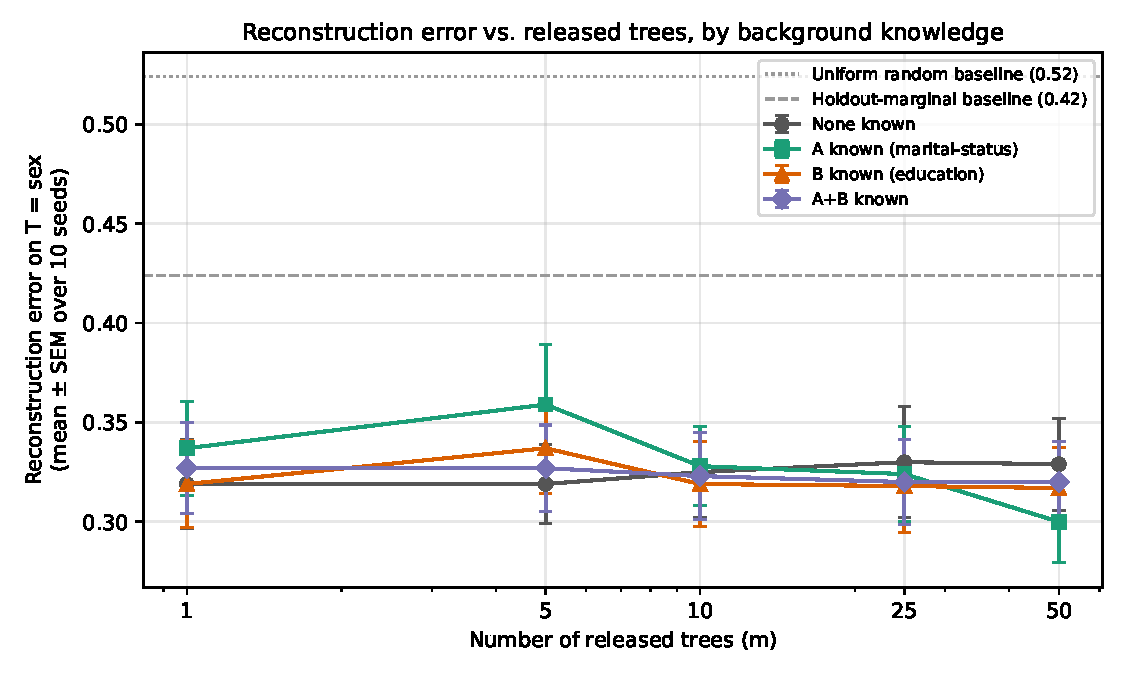
\includegraphics[width=0.85\textwidth]{figures/reconstruction_error_vs_m.pdf}
  \caption{Reconstruction error on $T=\texttt{sex}$ vs.\ number of released trees $m$, by background-knowledge condition. Error bars are $\pm 1$ standard error of the mean over 50 repetitions (fewer at $m=50,100$ where some repetitions' Rashomon sets or solves did not reach that point -- see Limitations).}
  \label{fig:error-vs-m}
\end{figure}

\paragraph{The released trees leak substantially more than either baseline.} All four conditions solve to error between $0.31$ and $0.36$ across every $m$ tested, against a uniform-random baseline of $0.50$ and a holdout-marginal baseline of $0.44$.

\paragraph{Background knowledge of $A$ and/or $B$ significantly reduces reconstruction error on $T$, with a clean ordering.} Unlike an earlier, shallower-tree version of this experiment, the four conditions now separate cleanly and consistently: $A{+}B < A \approx B < \text{None}$ at every $m$ from 10 onward (Table~\ref{tab:means}), and the gap widens as $m$ grows -- e.g.\ the $A{+}B$ advantage over \emph{None} grows from $0.013$ at $m=5$ to $0.025$ at $m=100$.

\begin{table}[h]
\centering
\begin{tabular}{lccccc}
\toprule
 & $m=5$ & $m=10$ & $m=25$ & $m=50$ & $m=100$ \\
\midrule
None & 0.350 & 0.358 & 0.342 & 0.343 & 0.337 \\
$A$    & 0.340 & 0.337 & 0.336 & 0.333 & 0.321 \\
$B$    & 0.343 & 0.343 & 0.345 & 0.333 & 0.322 \\
$A{+}B$ & 0.337 & 0.327 & 0.325 & 0.315 & 0.312 \\
\bottomrule
\end{tabular}
\caption{Mean reconstruction error on $T$ by condition and $m$.}
\label{tab:means}
\end{table}

A paired Wilcoxon signed-rank test (same seed and $m$, condition vs.\ \emph{None}), pooled across all $m$, confirms this is not noise:

\begin{center}
\begin{tabular}{lccc}
\toprule
 & $A$ & $B$ & $A{+}B$ \\
\midrule
mean difference vs.\ None & $-0.0127$ & $-0.0083$ & $-0.0228$ \\
$p$-value & $0.0013$ & $0.045$ & $4\times10^{-7}$ \\
\bottomrule
\end{tabular}
\end{center}

$A{+}B$ is also individually significant at $m=10$ ($p=0.006$), $m=50$ ($p=0.007$), and $m=100$ ($p=0.004$), and directionally negative (helps) at every $m$ tested. $A$ alone reaches significance at $m=10$ and $m=100$. $B$ alone is the weakest of the three: it is significant pooled, but at $m=25$ its mean difference is slightly \emph{positive} (i.e.\ knowing $B$ alone very slightly hurt reconstruction of $T$ in that slice of the data, $p=0.54$, not significant) before the expected direction reasserts itself at $m=50$ and $m=100$. We read this as $B$ (education, 5 categories) carrying a genuinely weaker and noisier signal about $T$ than $A$ (marital-status, 4 categories) in this sample, consistent with $A$ having a tighter empirical association with \texttt{sex} in Adult -- not as a failure of the method.

\paragraph{Why this result is stronger than an earlier pass of the same experiment.} An initial version of this experiment, run under a tighter compute budget, used regularization $\lambda=0.02$ and bound multiplier $0.2$, giving Rashomon sets of very shallow trees (1--3 splits) in which most trees never split on \texttt{sex} at all; the four conditions were statistically indistinguishable. The version reported here uses $\lambda=0.01$ (matching Hsu et al.'s own Adult setting) and a looser bound multiplier, giving substantially deeper trees (avg.\ depth 5.7) where \texttt{sex} is split on in essentially every tree and jointly with $A$/$B$ in the same root-to-leaf path in the large majority of trees. This supports the mechanism we hypothesized earlier: background knowledge only helps the attacker where a tree's structure directly entangles $T$ with the known attribute, and shallow trees simply don't create enough such entanglement to show an effect.

\paragraph{Limitations.} (i) The pooled Wilcoxon test treats each (seed, $m$) pair as an independent observation; the five $m$-values drawn from the same seed are not independent of each other (they reuse the same 100-row sample and overlapping trees from the same Rashomon set), so the pooled $p$-values should be read as a convenient summary rather than a fully rigorous combined test -- the per-$m$ tests, which are properly independent across seeds, are the safer basis for any claim. (ii) At $m=100$, the \emph{None} condition timed out (CP-SAT returned \texttt{UNKNOWN} within the 120s budget) for 9 of 50 repetitions, and 2 repetitions had Rashomon sets smaller than 50/100 trees and were excluded at those $m$ values entirely; $n$ at $m=100$ is therefore 39, not 50. (iii) The curated 13-column feature set, single enumeration-order tree selection (no diversity-aware strategy), and absence of a calibration/confidence measure remain as before.
